% % % % % % % % % % % % % % % % % % % % % 
% results.tex - Ian Huston
% $Id: results.tex,v 1.5 2009/10/05 15:52:09 ith Exp $
% % % % % % % % % % % % % % % % % % % % % 
% Redefine CVSRevision for this section
\renewcommand{\CVSrevision}{\version$Id: results.tex,v 1.5 2009/10/05 15:52:09 ith Exp $}

% % % % % % % % % % % % % % % % % % % % % % % % % % % % % % % % 
% =========================================================== %
% % % % % % % % % % % % % % % % % % % % % % % % % % % % % % % %
\chapter{Results and Future Work}
\label{ch:results}
% % % % % % % % % % % % % % % % % % % % % % % % % % % % % % % % 
% =========================================================== %
% % % % % % % % % % % % % % % % % % % % % % % % % % % % % % % %


% % % % % % % % % % % % % % % % % % % % % % % % % % % % % % % % 
% =========================================================== %
% % % % % % % % % % % % % % % % % % % % % % % % % % % % % % % %
\section{Results}
\label{sec:results}
% % % % % % % % % % % % % % % % % % % % % % % % % % % % % % % % 
% =========================================================== %
% % % % % % % % % % % % % % % % % % % % % % % % % % % % % % % %


The main result of this paper is the demonstration of a numerical solution to
the closed Klein-Gordon equation of motion for second order scalar field
perturbations as described in \eq{eq:KG2-fourier-sr-num}. This includes the slow
roll approximation of the source term for second order perturbations, but we
have not used a slow
roll version of the evolution equations for the background or first order
perturbations. 

As a proof of concept we have tested the system with two standard potentials,
$\msqphisq$ and $\lambdaphifour$ and computed results across three
different $k$ ranges. As expected, considering the use of a single slowly
rolling field, the second order perturbation we have calculated is extremely
small in comparison with the first order term. However there are already
differences apparent between the two potentials which will be outlined below.
We have calibrated the parameters $m$ and $\lambda$ of the potentials using the
WMAP 5 normalisation at $\kwmap=0.002 \Mpc^{-1} = 5.25 \e{-60}\Mpl$
\cite{Komatsu:2008hk}.
We have outlined in \eq{eq:Krangedefns} the three $k$ ranges that we will use,
% 
\begin{eqnarray*}
K_1 &=& \left[1.9\e{-5}, 0.039\right]\Mpc^{-1}\,,\quad \Delta k =
3.8\e{-5}\Mpc^{-1} \nonumber\\
K_2 &=& \left[5.71\e{-5}, 0.12\right]\Mpc^{-1}\,, \quad \Delta k =
1.2\e{-4}\Mpc^{-1}
\nonumber\\ 
K_3 &=& \left[0.52\e{-5}, 0.39\right]\Mpc^{-1}\,, \quad \Delta k =
3.8\e{-4}\Mpc^{-1} \,.
\end{eqnarray*}
Many of the results will be quoted for $\kwmap$ which lies in all three of these
ranges.

Given that the first order perturbations for the chosen potentials give an
almost scale invariant power spectrum with no running, it is no surprise that
the results from the three different $k$ ranges are very similar. The second
order source term is somewhat dependent on the lower bound of $k$ (upper bound
on size). This is expected and in the scale invariant case a log divergence can
be shown to exist \cite{Lyth:2007jh}. We have implemented an arbitrary sharp
cutoff at $\kmin$
below
which 
$\dvp1$ is taken to be zero. As mentioned above there is some evidence to
suggest that a 
similar cutoff is supported by the WMAP data \cite{Sinha:2005mn,Kim:2009pf}. 
% 
% % % % % % % % % % % % % % % % % % % % % % % % % % % % % % % % % % 

At first order our solutions agree with previous work
\cite{Salopek:1988qh,Martin:2006rs,Ringeval:2007am}, with oscillations
being damped until horizon crossing (when $k=aH$) after which the
curvature perturbation becomes conserved. Figure~\ref{fig:dp1} shows
the real and imaginary parts of the first order perturbations from
when the initial conditions are set at $k/aH=50$ to just after horizon
crossing. The x-axis for most of the following figures shows the
number of e-foldings left until the end of inflation instead of the
internally used time variable $\N$.
%
% 
\begin{figure}
 \centering
 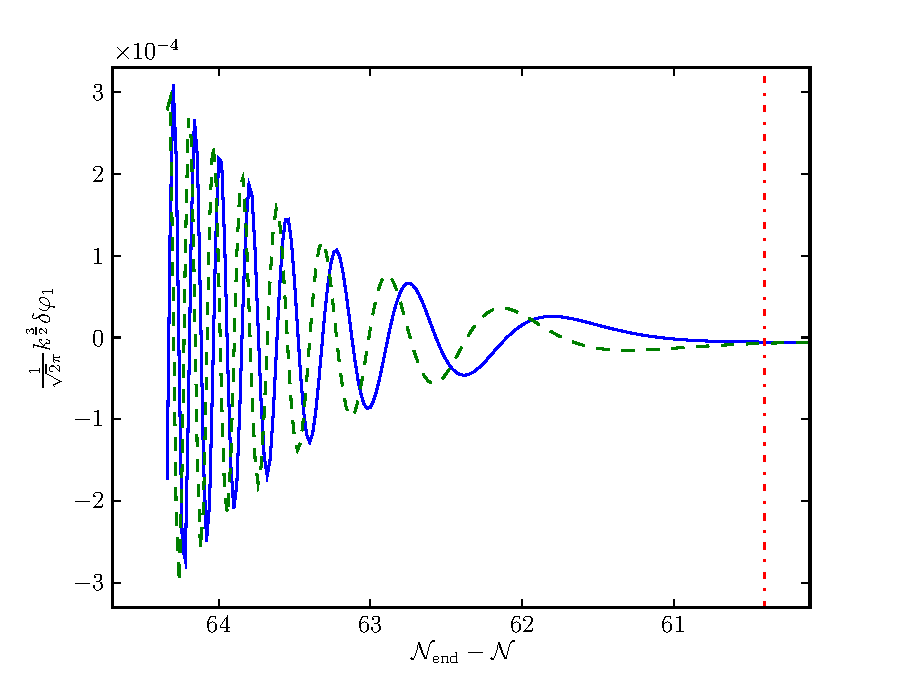
\includegraphics[width=\textwidth]{numerical/graphs/dp1_kwmap}
 \caption[First Order Perturbation]{The first order perturbation $\dvp1$ rescaled by
$k^{3/2}/(\sqrt{2}\pi)$ from the beginning of the simulation until around
horizon crossing (red dot-dashed line). The real (blue) and imaginary (green
dashed) perturbations are shown for $\kwmap$.}
\label{fig:dp1}
\end{figure}
% 
% % % % % % % % % % % % % % % % % % % % % % % % % % % % % % % % % % % 



In Figure~\ref{fig:dp2realimag} we show the evolution of the second
order perturbations for wavenumber $\kwmap$. As mentioned above the
overall amplitude of the second order perturbations is many orders of
magnitude smaller than the first order ones. In Figures~\ref{fig:dp1}
and \ref{fig:dp2realimag} the field values have been rescaled by
$k^{3/2}/(\sqrt{2}\pi)$ to allow a better appreciation of the
magnitude of the resulting power spectra.
% 
\begin{figure}
 \centering
 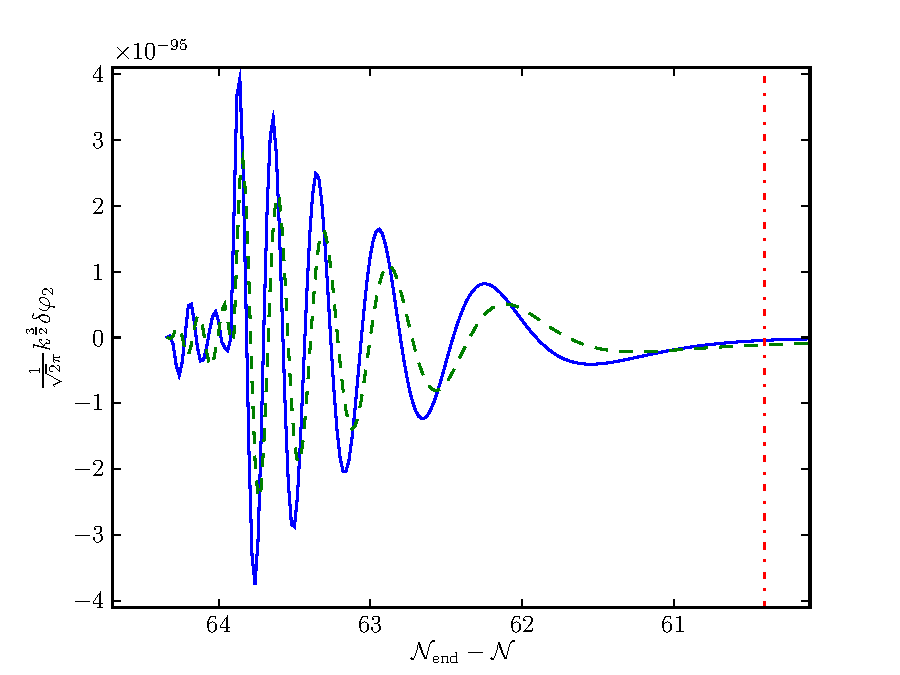
\includegraphics[width=\textwidth]{numerical/graphs/dp2_kwmap}
 \caption[Second Order perturbation]{The real (blue line) and imaginary (green
dashed) components of the
second order
perturbation $\dvp2(\kwmap)$ from the beginning of the simulation until around
the time
of horizon exit (red dot-dashed line).}
\label{fig:dp2realimag}
\end{figure}
% 
% % % % % % % % % % % % % % % % % % % % % % % % % % % % % % % % % % % 



The source term $S(\kvi)$ is calculated at each time step using the
results of the first order and background runs. This term drives the
production of second order perturbations as shown in
\eqs{eq:KG2-fourier-sr-num} and
(\ref{eq:KG2-fourier-sr-ntime}). Figure~\ref{fig:src-full} shows the
absolute magnitude of the source term for a single $k$ mode, $\kwmap$,
for all time steps calculated.
% 
\begin{figure}
\centering
\subfloat[Absolute magnitude of the source term.]{
 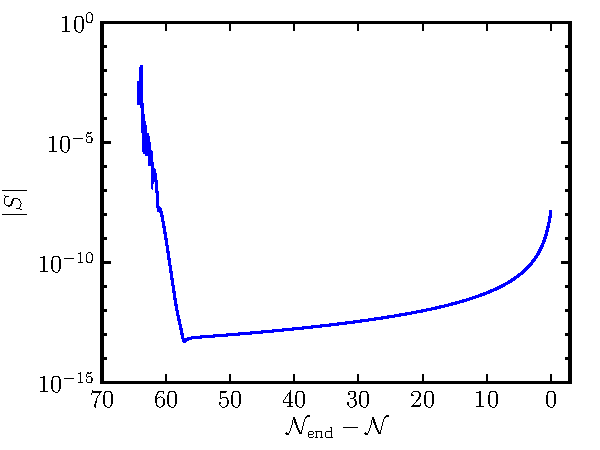
\includegraphics[width=0.43\textwidth]{numerical/graphs/src-kwmap-small}
\label{fig:src-full}
}\qquad
% 
\subfloat[Power spectrum of scalar perturbations][Power spectrum of scalar
perturbations $\mathcal{P}_{\delta\varphi} =
\frac{k^3}{2\pi^2}|\delta\varphi|^2$.]{
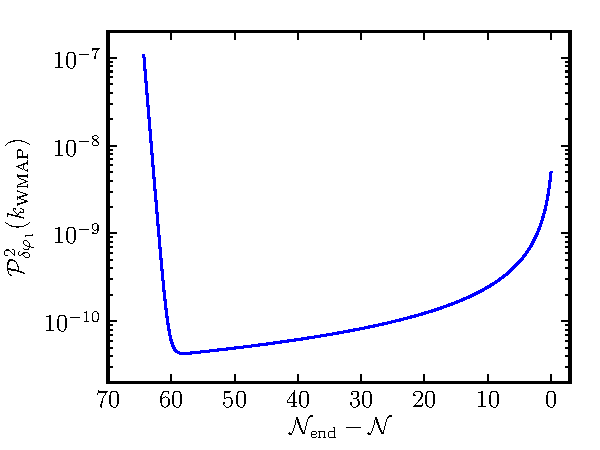
\includegraphics[width=0.43\textwidth]{numerical/graphs/Pphi-kwmap-nohoriz-small}
\label{fig:Pphi-kwmap}
}
\caption[The source term and power spectrum for $\kwmap$]{Source term and power
spectrum for the WMAP pivot scale $\kwmap$.}
\end{figure}
% 
Figure~\ref{fig:src-kwmap-3ranges} shows how the source term changes
with the choice of $k$ range.  After horizon crossing the source terms
are approximately equal. Before horizon crossing however there is a
strict hierarchy with the smaller $k$ ranges, $K_1$ and $K_2$, leading to
smaller source
contributions.  As stated in Section \ref{sec:codetests}, $\Delta k$
should be at least as large as $\kmin$ in order to reduce the error to
a minimum.
% 
\begin{figure}
\centering
 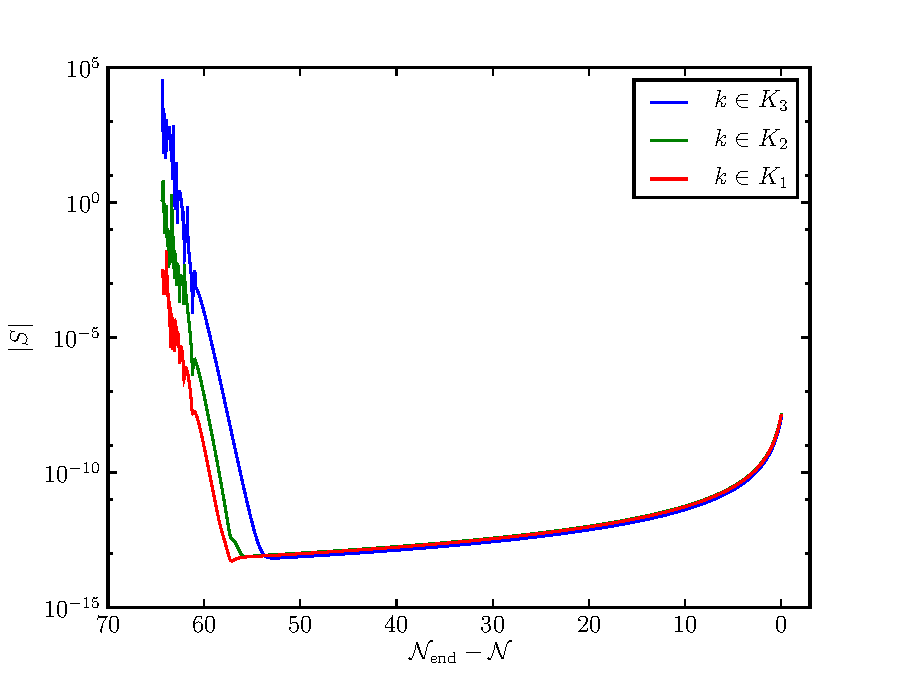
\includegraphics[width=\textwidth]{numerical/graphs/src-kwmap-3ranges-large}
\caption[Comparison of source term for different ranges]{Comparison of the source
term for $\kwmap$ over three different ranges with different $\Delta k$s as specified
in
\eq{eq:Krangedefns}.} 
\label{fig:src-kwmap-3ranges}
\end{figure}
% 
\begin{figure}
\centering
 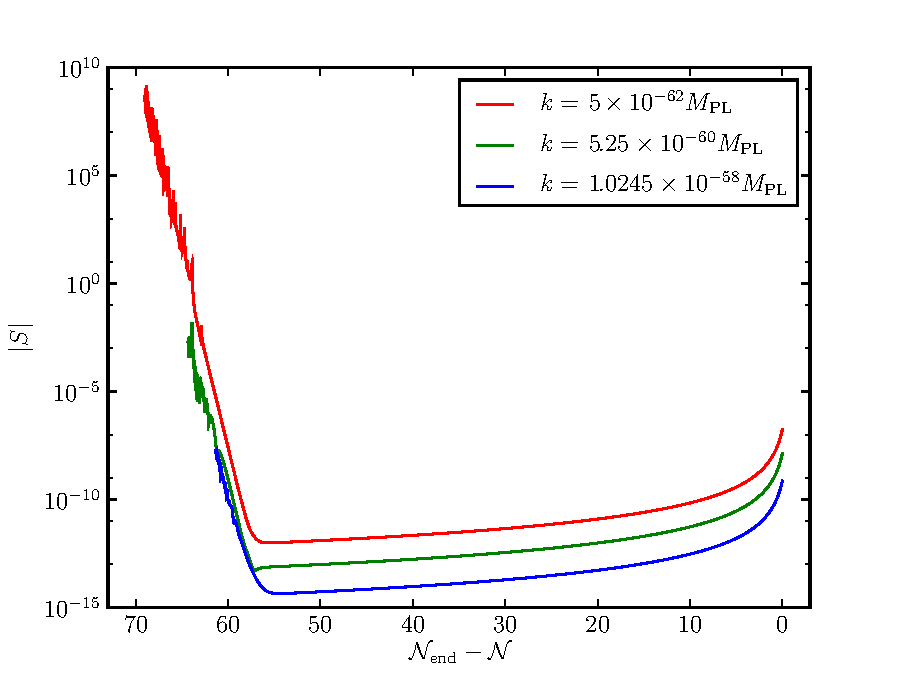
\includegraphics[width=\textwidth]{numerical/graphs/src-3ks-large}
\caption[Source term at three different $k$s]{The source term for three different $k$
values including the WMAP
pivot scale. As $k$
gets larger (scale gets smaller) the source term becomes smaller.}
\label{fig:src-3ks}
\end{figure}
% 
% 



The source term is large at early times, and closely follows the form
of the spectrum of the first order perturbations as can be seen from
Figure~\ref{fig:Pphi-kwmap}.
%
It is useful to compare the magnitude of the source term with the
other terms in the second order evolution equation
(\ref{eq:KG2-fourier-sr-ntime}). If we let $T$ denote the other terms,
%
\begin{equation}
\label{eq:Tdefn}
 T(\kvi) = \left(3 + \frac{\dN{H}}{H}\right)
\dN{\dvp2}(\kvi)+ \left(\frac{k}{aH}\right)^2\dvp2(\kvi)
+\left(\frac{\Upp}{H^2}-{24 \pi G}(\dN{\vp_{0}})^2\right)
\dvp2(\kvi) \,,
\end{equation}
%
then Figure~\ref{fig:src-vs-others} shows the absolute magnitude of
both $S$ and $T$.  It is clear that the source term is of comparable
magnitude only early in the simulation.  Figure~\ref{fig:s-over-t-3ks}
shows a comparison of $|S|/|T|$ for three different $k$ values. The larger the
$k$ mode the closer
in amplitude $S$ is to the rest of the terms in the ODE.
A priori it is not known
where $S$ will be large for a particular chosen potential and mode but
once determined it could be possible to significantly reduce the time required
for the simulation by only calculating $S$ in the regions where it is
important.
%
\begin{figure}
\centering
 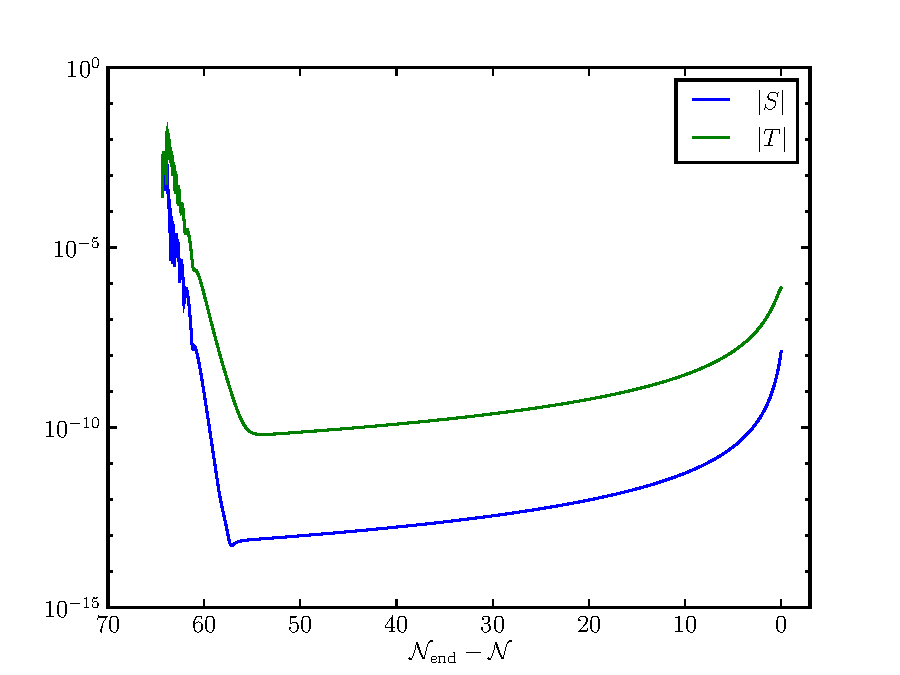
\includegraphics[width=\textwidth]{numerical/graphs/src-vs-t-kwmap-large}
\caption[Source term compared to $T$ term]{The source term (lower blue line) is
compared with the $T$ term
(upper green line) as defined in the text for $\kwmap$. The source term is of
comparable magnitude at the beginning of the simulation.}
 \label{fig:src-vs-others}
\end{figure}
% 
\begin{figure}
\centering
 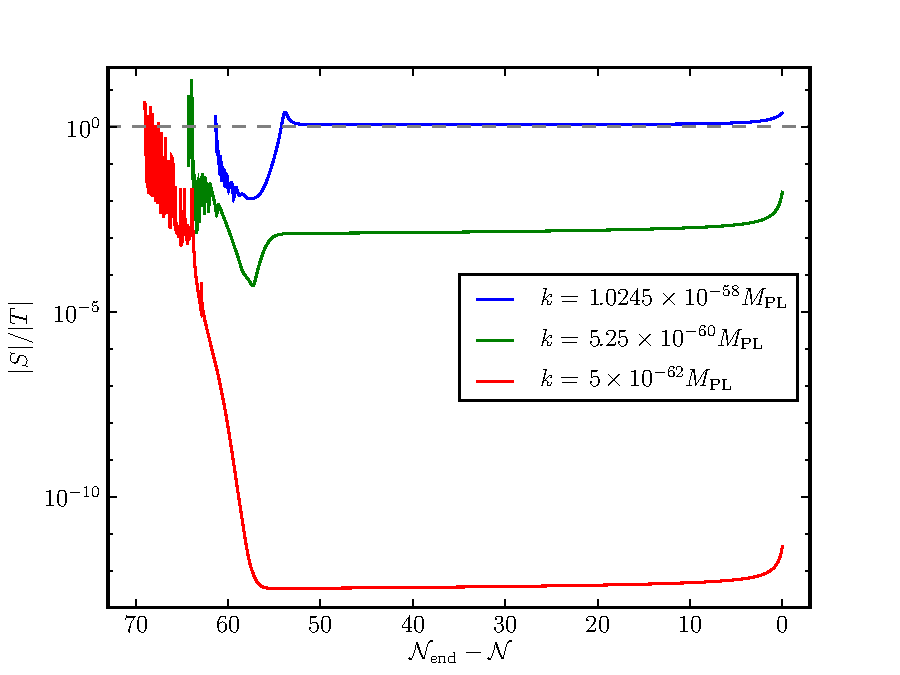
\includegraphics[width=\textwidth]{numerical/graphs/s-over-t-3ks-large}
\caption[Quotient of $S$ and $T$]{The quotient of $S$ and $T$ terms for three
different $k$ values
including the WMAP pivot scale. Depending on $k$ the source term only dominates
at early stages or is important throughout the evolution.}
 \label{fig:s-over-t-3ks}
\end{figure}
% 
% 
% % % % % % % % % % % % % % % % % % % % % % % % % % % % % % % % % % 


All the results quoted so far are for
the $\msqphisq$ model. We have also tested the $\lambdaphifour$ model and
compared it to
$\msqphisq$. Figure~\ref{fig:src-mvl-main} compares the models for $\kwmap$.
Figure~\ref{fig:src-mvl-zoom} shows how the source term for the $\lambdaphifour$
model is larger
than the one for $\msqphisq$ to begin, but crosses over after a few e-foldings.
After horizon
crossing the $\lambdaphifour$ source term is again larger. As the results at
first order for both
models are so similar it is to be expected that the second order perturbations
would be closely
related. 
% 
\begin{figure}
\centering
 \subfloat[Comparison of full evolution][The $\lambdaphifour$
model (green dashed line) initially has a
larger source term but becomes smaller than the $\msqphisq$ model as evolution
continues. After horizon crossing the $\lambdaphifour$ term is slightly
larger.]{
 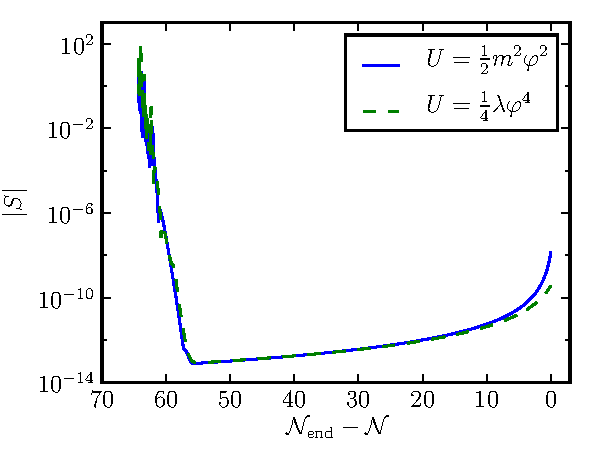
\includegraphics[width=0.43\textwidth]{numerical/graphs/src-mvl-small}
 \label{fig:src-mvl}
}\qquad
% 
\subfloat[Comparison at early times][The crossover between the models at the early
stages of the
simulation, before horizon 
crossing.]{
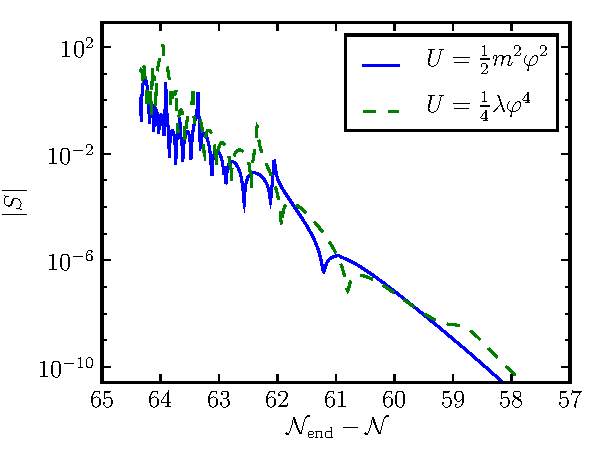
\includegraphics[width=0.43\textwidth]{numerical/graphs/src-mvl-zoom-small}
\label{fig:src-mvl-zoom}
}
\caption[Comparison of the $\lambdaphifour$ and $\msqphisq$ models]{A comparison of 
the source term for the $\msqphisq$ and $\lambdaphifour$ models.}
\label{fig:src-mvl-main}
\end{figure}
% 
% % % % % % % % % % % % % % % % % % % % % % % % % % % % % % % % % % %

In Figure~\ref{fig:src-kinit} the value of $|S|$ at the start of the evolution
of $\dvp2$ for
each $k$ mode is shown. The magnitude of the source term is much smaller for
larger $k$s (smaller
scales). 
Because the smaller $k$s begin their evolution earlier the relative difference
in $|S|$ is not as
pronounced when measured at a single timestep (see for example
Figure~\ref{fig:src-3ks}).
It should also be remembered that the magnitude of other terms in the second
order ODE is
small for larger $k$s as shown by the ratio $|S|/|T|$ in
Figure~\ref{fig:s-over-t-3ks}
where $T$ is defined above in \eq{eq:Tdefn}.
\begin{figure}
\centering
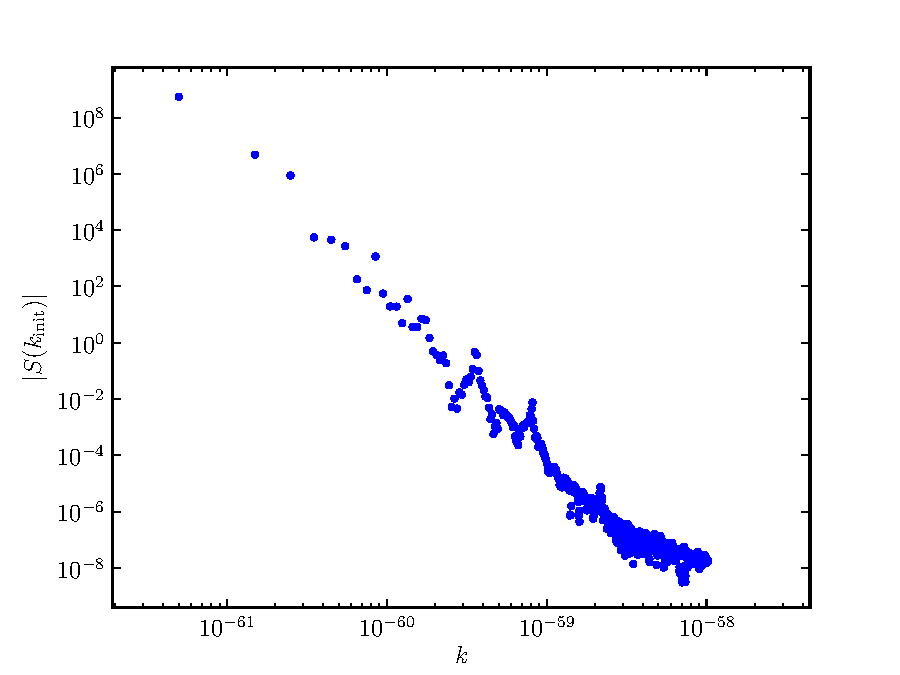
\includegraphics[width=\textwidth]{numerical/graphs/src_kinit_log}
 \caption[Source term at initial start times]{The absolute magnitude of the source 
term at the initial start time for each $k$ when $k = aH \times 50$ deep inside the
horizon. The results are for the range $K_1=\left[ 1.9\e{-5},
0.039 \right] \Mpc^{-1}= \left[0.5\e{-61}, 1.0245\e{-58}\right]\Mpl$.}
\label{fig:src-kinit}
\end{figure}
% 

The source term for all $k$s can also be compared for different timesteps. In
Figure~\ref{fig:src-3ns} the upper blue line shows $|S(k)|$ around 69 e-foldings
before the end of
inflation when $\dvp2$ has been initialised for only the very smallest $k$
modes. The middle green
line shows $|S|$ when all $\dvp2$ modes have been started. Finally the lower red
line plots $|S|$
after all modes have exited the horizon, around 52 e-foldings before the end of
inflation.
\begin{figure}
\centering
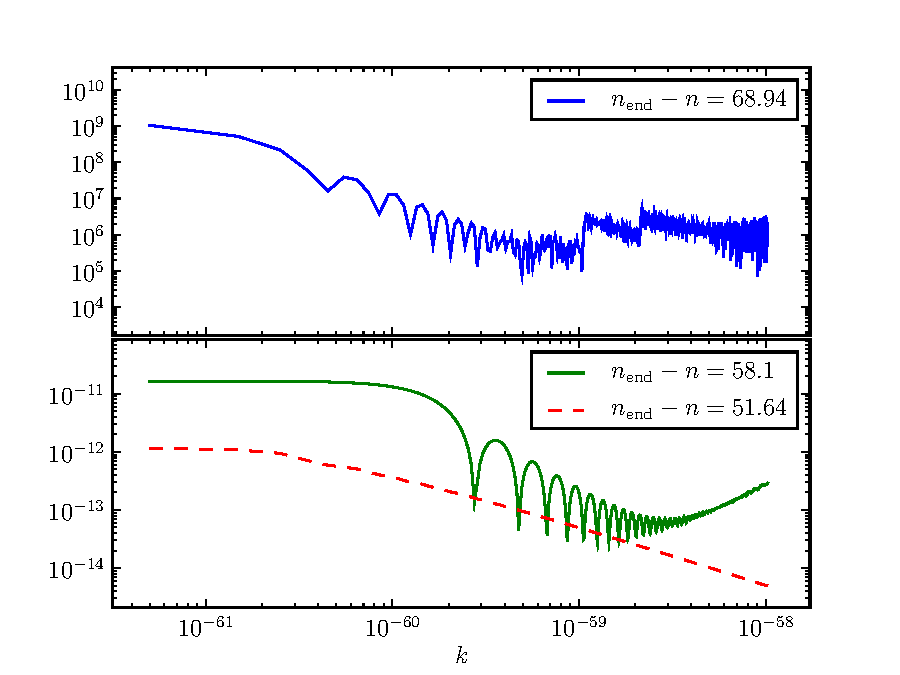
\includegraphics[width=\textwidth]{numerical/graphs/src_3ns}
\caption[Source term at three different times]{The absolute magnitude of the source 
term for all $ks$ in the range at three different timesteps: the upper blue line when
only the largest modes have been initialised; the middle green line when all modes
have been initialised; and the lower red dashed line when all modes have
exited the horizon. The $k$ range shown here is $K_1=\left[ 1.9\e{-5}, 0.039
\right] \Mpc^{-1}= \left[0.5\e{-61}, 1.0245\e{-58}\right]\Mpl$.}
\label{fig:src-3ns}
\end{figure}
% 
% % % % % % % % % % % % % % % % % % % % % % % % % % % % % % % % 

% % % % % % % % % % % % % % % % % % % % % % % % % % % % % % % % 
% =========================================================== %
% % % % % % % % % % % % % % % % % % % % % % % % % % % % % % % %
\section{Next steps}
\label{sec:next-res}
% % % % % % % % % % % % % % % % % % % % % % % % % % % % % % % % 
% =========================================================== %
% % % % % % % % % % % % % % % % % % % % % % % % % % % % % % % %

% 
% 
% 
% % % % % % % % % % % % % % % % % % % % % % % % % % % % % % % % 
% =========================================================== %
% % % % % % % % % % % % % % % % % % % % % % % % % % % % % % % %
\section{Discussion and conclusion}
\label{sec:disc-num}
% % % % % % % % % % % % % % % % % % % % % % % % % % % % % % % % 
% =========================================================== %
% % % % % % % % % % % % % % % % % % % % % % % % % % % % % % % %

In this paper we have described the numerical solution of the
evolution equations for second order scalar perturbations, using the
closed form of the Klein-Gordon equation, \eq{eq:KG2-fourier-sr-num}. We
demonstrate that direct calculation of field perturbations beyond
first order using perturbation theory is readily achievable, though
not trivial.

For this first demonstration we have limited ourselves to considering
the slow roll source term in \eq{eq:KG2-fourier-sr-num} but without imposing
slow roll on the evolution terms of the ODEs. We have investigated two
standard potentials, $\frac{1}{2}m^2\phi^2$ and
$\frac{1}{4}\lambda\phi^4$, to demonstrate the capabilities of the
system. The singularity at $k=0$ which arises as larger and larger
scales are considered is avoided by implementing a cutoff at small
wavenumbers below $\kmin$. This is a pragmatic choice necessary for
the calculation, but as mentioned above there is some evidence that
such a cutoff might also explain lack of power at large scales in the
WMAP data \cite{spergel, Sinha:2005mn, Kim:2009pf}. It is also necessary to
pick a maximum $k$ value, and this choice is dictated by computational
resources and with reference to observationally relevant scales. In
this paper we have used $k$ ranges which are comparable with the
scales observed by WMAP. By comparing the analytical results of the
convolution integral with the numerical calculation, we have chosen
values of the parameters $N_\theta, N_k$ and $\Delta k$ which minimise
the numerical error. The convolution scheme that we have implemented
works best when $\Delta k>\kmin$.


We have shown explicitly that the second order calculations for our chosen
potentials are obtainable once the cut-off for $\kmin$ is
implemented. As expected for these unexceptional potentials in the slowly
rolling regime the magnitude of second order perturbations is extremely
suppressed in comparison with the first order amplitude. We have shown the
evolution of the source term equation during the inflationary regime can be
readily calculated.


There are many possible next steps to improve the program outlined in
Section \ref{sec:numerics}. Chief amongst these is to implement the
full source term equation (\ref{eq:KG2-source-ntime}). Although clearly
more complicated than the slow roll case in \eq{eq:KG2-fourier-sr-ntime}
only two more $\theta$ dependent terms need to be added to $A$--$D$ in
\eq{eq:AtoD-num}.  For the two test models we have used in this paper, which
are both slowly rolling during inflation, it is not expected that
using the full source equation would result in an appreciably
different outcome until the end of the inflationary phase. Though once
the field has stopped to roll slowly, new observable features might
arise as is indeed the case at first order. 


Beyond this the next likely step is to implement a multi-field version of the
system. This would allow the investigation of models that inherently
produce large second order perturbations. In Ref.~\cite{Malik:2006ir} the
Klein-Gordon equation is given for multiple fields and upgrading the
simulation to use these equations is a
straight-forward if lengthy process.  


The performance of the numerical simulation could also be improved by
analysing the most time consuming processes and investigating what
optimisations could be implemented. As we have discussed above we have
set $N_k=1025$ for our test runs. This provides good coverage of the
WMAP $k$ range but it is not clear whether it sufficiently
approximates the integral to infinity for the source term.  Currently
we are restricted in our choice of $N_k$ by logistical factors \ie the
running time and memory usage of the code. By optimising the routines
for both memory and speed it is hoped we can extend the maximum value
of $k$ to larger values.


By computing the perturbations to second order we have direct access
to the non-gaussianity of $\dvp{}$.  While useful for the toy models
discussed above (with $\fnl\simeq0$), when used to investigate models
with predictions of large non-linearity parameter $\fnl$ this technique
could yield greater insight into the formation and development of the
non-gaussian contributions by studying the contribution of the different
terms in the source term \eq{eq:KG2-source-ntime}.
%
It was shown recently that in order to calculate $\fnl$ instead of
using the standard method based on the Lagrangian formalism
\cite{Maldacena:2002vr}, one can instead use the field equations
\cite{Musso:2006pt,Seery:2008qj}. The method presented here will
therefore eventually allow a full numerical calculation of $\fnl$.


In summary, we have demonstrated that numerically solving the closed
Klein-Gordon equation for second order perturbations is possible. We
have used the slow roll version of the source term in this paper, but
hope to extend our work to use the full source soon. The two test
models we have used have been shown to have negligible second order
perturbations in line with analytic results. We have compared the
analytic and numerical solutions for the convolution term and found
them to be in good agreement.
